%%%%%%%%%%%%%%%%%%%%%%%%%%%%%%%%%%%%%%%%%%%%%%%%
%%%%%%%%%%%%%Przykładowy dokument%%%%%%%%%%%%%%%
%%%%%%%%%%wraz z klasą pracadyp.cls%%%%%%%%%%%%%
%%%%%%%%%%%%%%%%%%%%%%%%%%%%%%%%%%%%%%%%%%%%%%%%

% w nawiasie kwadratowym wpisujemy rodzaj pracy: 
% magisterska, licencjacka, inzynierska
\documentclass[licencjacka]{pracadypl}


%% ważne definicje %%
\usepackage{tgtermes}
\usepackage[T1]{fontenc}
\usepackage{polski}
\usepackage[utf8]{inputenc}
\input glyphtounicode
\pdfgentounicode=1
\usepackage{amssymb}
\usepackage{amsmath}
\usepackage{graphicx}
\usepackage{titlesec}
\usepackage{color}
\usepackage{xcolor}
\usepackage{float}
\usepackage{tablefootnote}
\usepackage{hyperref}
\usepackage{titling}
\bibliographystyle{plain}

\def\mgr{magisterska}
\def\lic{licencjacka}
\def\inz{inżynierska}

\def\sk{Słowa kluczowe}
\def\kw{Keywords}
\def\et{Title in English}
%% koniec ważnych definicji %%



%% wypełnia Autor pracy %%

%autor pracy
\author{Kajetan Owczarek}
%numer albumu
\nralbumu{396396}
%tytuł pracy
\title{Przykłady zastosowania technik optymalizacji czasu wczytywania witryny internetowej}
%kierunek studiów
\kierunek{Informatyka}
%promotor w dopełniaczu
\opiekun{prof. dr Wojciecha Horzelskiego}
\katedra{Katedra Informatyki Stosowanej}
%rok
\date{2023}
%Słowa kluczowe:
\slkluczowe{pierwsze, drugie, trzecie, czwarte}
%tytuł po angielsku
\tytulang{Title in English}
%słowa kluczowe po angielsku
\keywords{first, second, third, fourth}
%% koniec ważnych definicji %%

%% APD %%
%% w systemie APD należy jeszcze wpisać, poza powyższymi informacjami, streszczenie oraz streszczenie w języku angielskim  %%


%%% definicje %%%
\def\pd{\noindent \textbf{Dowód.~}} %%początek dowodu
\def\kd{\hfill\mbox{$\rule{2mm}{2mm}$}} %%koniec dowodu
\newtheorem{defi}{Definicja}[section]
\newtheorem{uwaga}{Uwaga}[section]
\newtheorem{tw}{Twierdzenie}[section]
\newtheorem{lem}{Lemat}[section]
\newtheorem{wn}{Wniosek}[section]
\renewcommand\thetw{\thesection.\arabic{tw}.}
\renewcommand\thedefi{\thesection.\arabic{defi}.}
\renewcommand\theuwaga{\thesection.\arabic{uwaga}.}
\renewcommand\thetw{\thesection.\arabic{tw}.}
\renewcommand\thelem{\thesection.\arabic{lem}.}
\renewcommand\thewn{\thesection.\arabic{wn}.}
%
\definecolor{wmiigreen}{rgb}{0.0, 0.5, 0.0}
\titleformat{\chapter}[display]
  {\normalfont\huge\bfseries\color{wmiigreen}}{\chaptertitlename\ \thechapter}{10pt}{\Huge}
 %
\linespread{1.3}
%%% koniec definicji ze wzorca %%%


%%% osobiste definicje

\newcommand{\selfnote}[1]{\colorbox{pink}{#1}}
\hypersetup{
  colorlinks=false,
  linkcolor=red,
  pdftitle={\thetitle},
  pdfborder={0 0 0}
}

%%% koniec definicji

\begin{document}

\maketitle
\tableofcontents
\newpage



\chapter{Wstęp}

Pomimo nieustającego rozwoju technologii telekomunikacji oraz zwiększania prędkości łączy internetowych, problem wydajności usług internetowych nie zniknął, ani nie zapowiada się, aby tak się zadziało. Od potrzeb łączności poza terenami zabudowanymi, przez starzejący lub ograniczony sprzęt, po malejącą cierpliwość użytkowników, rozważanie, jak najszybciej dostarczyć treści z serwera do urządzenia użytkownika jest powszechne w pracy ze stronami internetowymi.

Celem tej pracy jest zaprezentowanie serii technik i optymalizacji, pozwalających na poprawienie czasów wczytywania witryn internetowych na urządzeniach użytkownika, oraz porównanie ich przy pomocy obiektywnych i powszechnie stosowanych narzędzi i metryk.

Celem zilustrowania efektów takich optymalizacji, a w szczególności wpływ ich braku na używalność strony, zaprezentuję przykładową stronę zrobioną przy użyciu najprostszych, najpopularniejszych technik. Celem moim jest stworzenie strony, która zrobiona jest kompetentnie, acz z zerową uwagą przyłożoną do wydajności strony pod względem wczytywania i procesu uruchamiania strony. Następnie, poprzez stosowanie technik wpływających minimalnie na funkcjonalność strony, poprawiać wyniki pomiarów obiektywnych.

\chapter{Sposób pomiarów}
Celem usunięcia jak najwięcej zewnętrznych zmiennych w danych pomiarowych,
% \footnote{Choć dla porównania wydajności wyniki z jednej maszyny powinny wystarczyć, niestety zaobserwowałem znaczne, trudne do zrozumienia fluktuacje wydajności mojego komputera. Wyniki na nim były by więc wewnętrznie niespójne.}
skorzystam z narzędzia używanego powszechnie w branży, którym jest WebPageTest.

WebPageTest to operowana przez firmę Catchpoint usługa, pozwalająca na wykonanie dokładnego pomiaru wczytywania strony w wybranym regionie, na emulowanym urządzeniu, w określonych warunkach sieciowych. Używając standaryzowanego środowiska, możemy usunąć wiele zmiennych wynikających z aktywności innych aplikacji na testującej maszynie oraz innych urządzeń w sieci. Sprawia to też, że wyniki są o wiele bardziej uniwersalne - mogąc odnieść się do środowiska ze znanymi charakterystykami wydajności, można usunąć element niepewności i zgadywania, na ile aplikowalne są dla naszych rozważań czyjeś wyniki. 

WebPageTest dostarcza dokładny zapis procesu wczytywanie naszej witryny. Dane te są prezentowane w formie złożonego wykresu, o którym opowiem więcej w późniejszym rozdziale, kiedy zajmiemy się porównywaniem wydajności przed i po zastosowaniu technik.

Rozważałem wcześniej użycie do pomiarów stworzonego przez Google narzędzia o nazwie Lighthouse, które stara się spełnić podobną funkcję oceny wydajności, acz analizuje też wiele innych metryk dotyczączych rzeczy jak używanie technologii pomagających osobą używającym czytników ekranu, optymalizacji pod kątem wyszukiwarek internetowych, czy współczesności strony. Niestety, sposób działania Lighthouse'a jest ograniczony w swojej dokładności. Zamiast dokonywać pełnej symulacji wydajności standardowego urządzenia, dokonuje on testy w pełnej prędkości, a następnie przeskalowując je. Tak jak nie jest to zła metoda żeby optymalizować lokalnie, gdyż Lighthouse sugeruje też sposoby poprawy, tak użycie go nie eliminuje częściowej zmienności wynikających z natury maszyny, na którym są dokonywane pomiary.

\chapter{Startowy projekt}
Żeby zilustrować techniki, które zostaną omówione później, oraz ich wpływ na wydajność wczytywania strony, potrzebna jest na to przestrzeń w formie przykładowej witryny. Tworząc ją, celowałem w popełnienie prostych do popełnienia błędów, oraz decyzje niesprzyjające czasowi wczytywania. Stworzyłem więc udawaną stronę z wiadomościami. Zawiera ona niemałą ilość zdjęć, dużo tekstu, oraz parę elementów interaktywnych. 

\begin{figure}[H]
  
\includegraphics[width=\linewidth]{images/frontpage.png}
  \caption{Nagłówek strony, karuzela z wiadomościami}
  \label{fig:frontpage}
\end{figure}

\begin{figure}[H]
  
\includegraphics[width=\linewidth]{images/frontpage-articles.png}
  \caption{Fragment listy artykułów}
  \label{fig:frontpage-articles}
\end{figure}

\begin{figure}[H]
  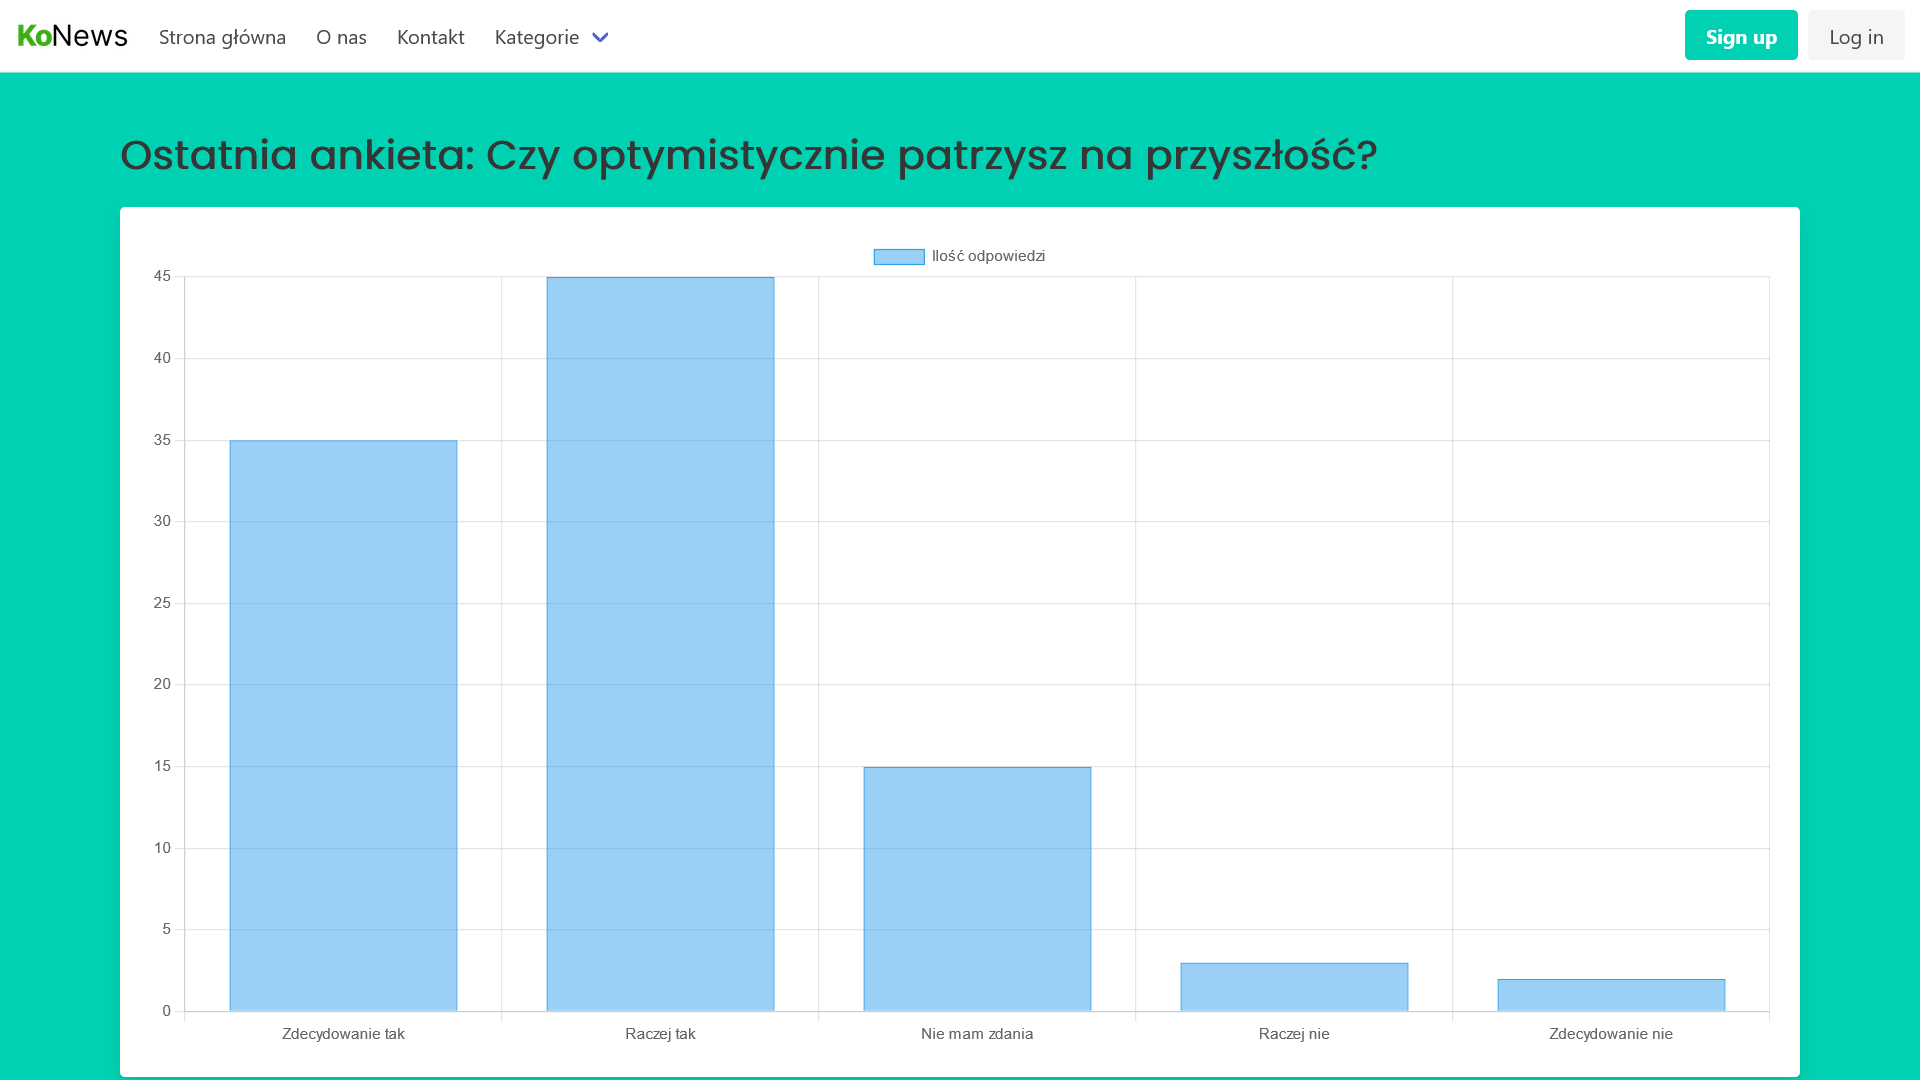
\includegraphics[width=\linewidth]{images/frontpage-dynamic-article.png}
  \caption{Dynamiczne treści - wyniki ankiety w wykresie}
  \label{fig:frontpage-dynamic}
\end{figure}

Żeby zaprezentować efekty dużej ilości treści w dokumencie HTML, dodałem do niej jedno ze źródeł do treści tu zawartej, czyli specyfikację parsowania dokumentów HTML.

\begin{figure}[H]
  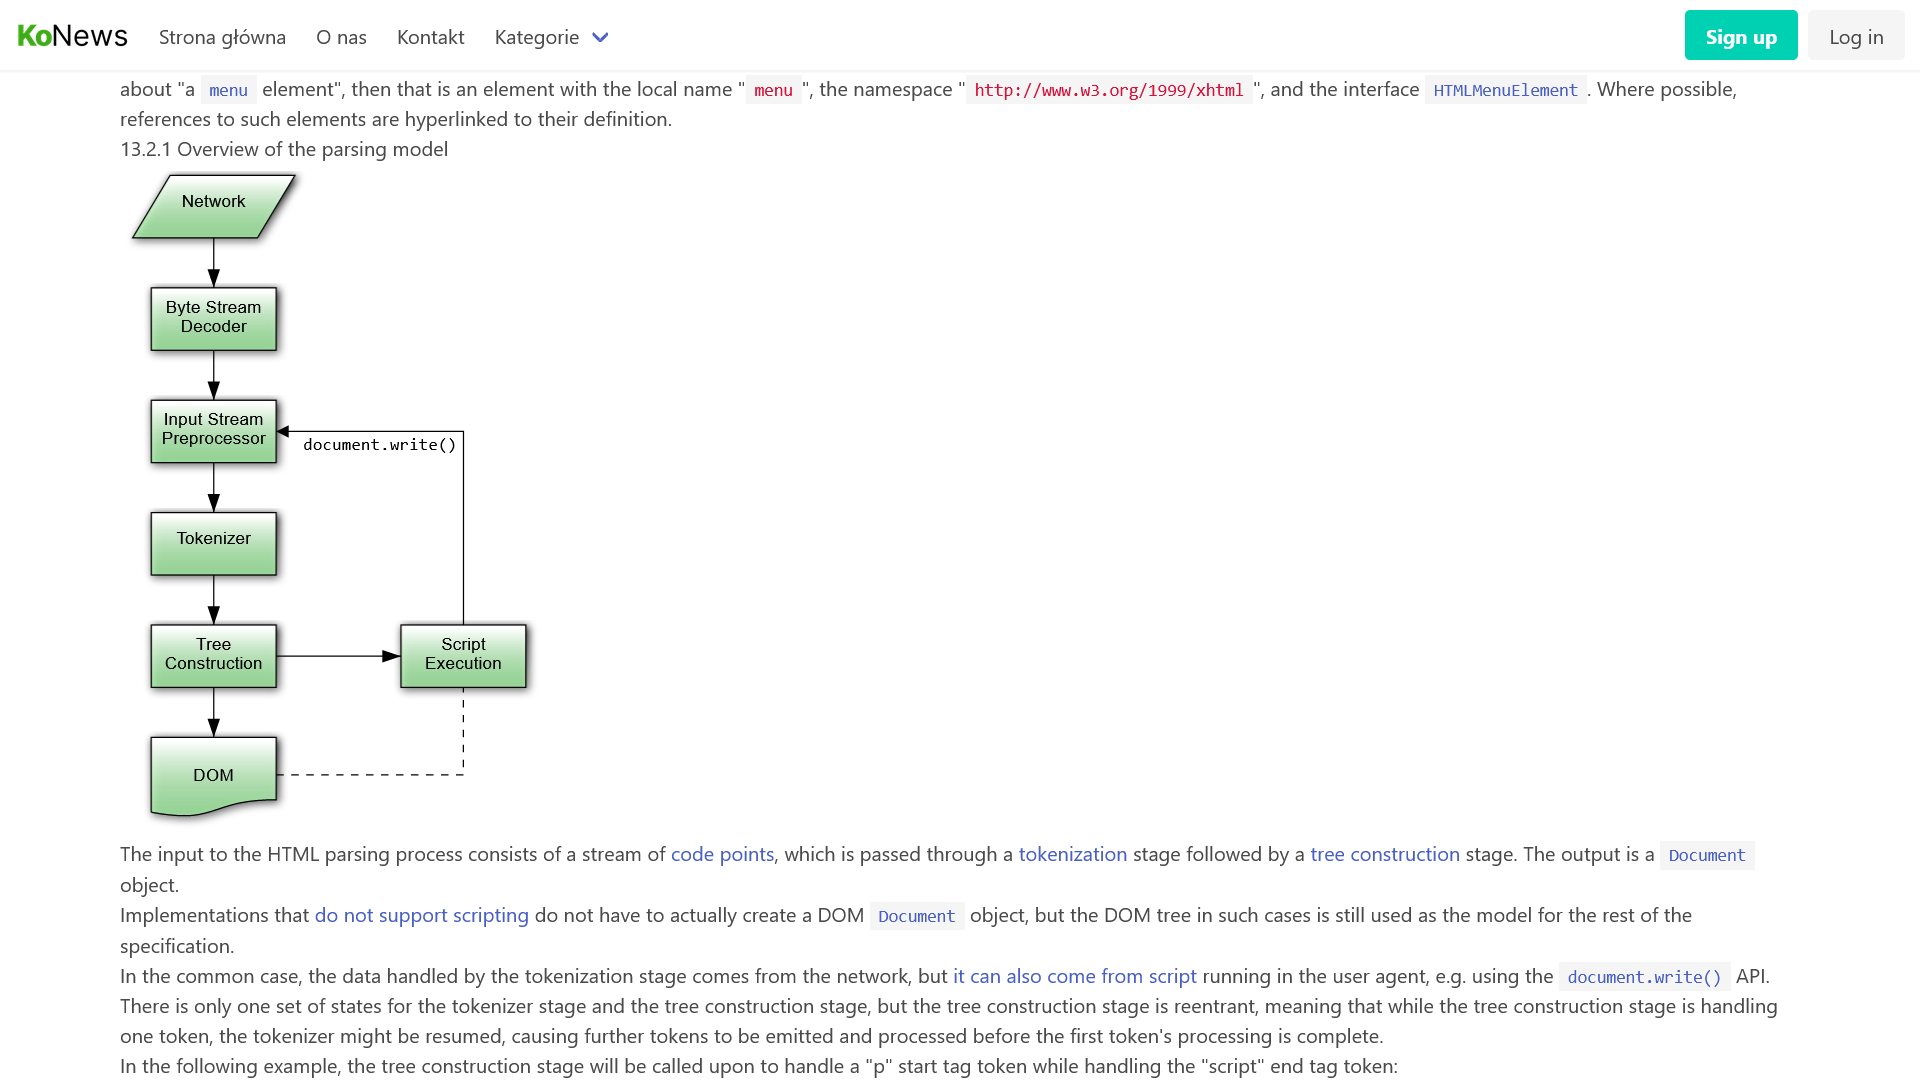
\includegraphics[width=\linewidth]{images/frontpage-spec.png}
  \caption{Duże treści - specyfikacja parsowania HTML}
  \label{fig:frontpage-spec}
\end{figure}




\chapter{Wstępna analiza wydajności}
Zanim zaczniemy poprawianie naszej witryny, powinniśmy zbadać, jak zachowuje się nasz projekt startowy. Optymalizując na ślepo, jest prosto zmarnować czas przyśpieszając elementy, nie zmieniając finalnej wydajności\footnote{W przypadku tworzenia witryn internetowych jest to szczególnie prosty do popełnienia błąd. Interakcja równoległego wczytywania zasobów, oraz mechanizm zasobów blokujących może sprawić, że dowolne przyśpieszenie jednej cześci nie wpłynie zupełnie na finalną szybkość wczytania, gdyż całość przeglądarki będzie czekało na inny element.}. Głownym wynikiem wykonywania analiz przy pomocy WebPageTest'u jest wykres zwany waterfall'em, czyli wodospadem. Jest on bardzo gęsty w dane i zawiera przede wszystkim dane o połączeniach sieciowych oraz stanie przeglądarki. Omówię po krótce jak go odczytywać\footnote{Dostepna na stronie WebPageTest'u lekko interkatywna wersja tego wykresu pozwala odczytać te dane nieco prościej, oraz daje dostęp do dodatkowych informacji, których nie ma na obrazkowym waterfall'u.}, równocześnie zwracając uwagę na problemy, które można zobaczyć ze wstępnych testów;
\begin{figure}[h!]
  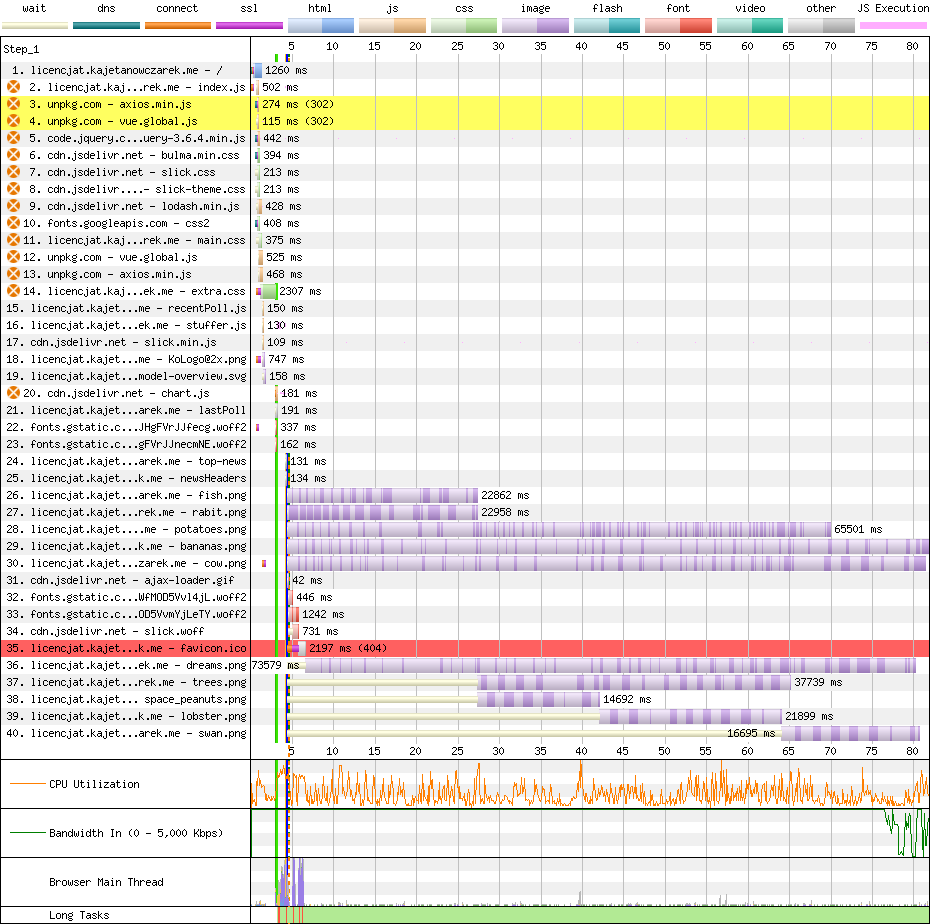
\includegraphics[width=\linewidth]{images/base-waterfall-all-final.png}
  \caption{Wykres produkowany przez WebPageTest, zwany jako Waterfall}
  \label{fig:waterfall-base}
\end{figure}
Na górze wykresu znajduje się legenda, informująca nas, które kolory na wykresie oznaczają jaką fazę rozpoczynania połączeń, oraz rodzaje treści przez te połączenia przesyłane. 

Tuż pod nią, znajduje się głowna część, która zawiera najważniejsze dane, czyli wykres rozkładu czasowego realizacji kolejnych zapytań wykonywanych przez naszą przeglądarkę. Od góry do dołu mamy zapytania HTTP, od rozpoczętego najwcześniej do najpóźniej, natomiast od lewej do prawej mamy upływ czasu. Same okresy, kiedy zapytania naszej witryny były realizowane, są zaznaczone jako prostokąty na wykresie. Poprzez cienkie prostokąty są zaznaczane obszary czasu, kiedy połączenia nie postępowały stan wczytania naszej strony, specyficznie otwieranie połączeń i wykonywanie kodu JavaScript. Grubymi prostokątami jest za to zaznaczone, kiedy treści rzeczywiście były pobierane, na blado kiedy połączenie jest otwarte, ale nie są przesyłane dane, oraz na mocniejszy kolor, kiedy miało miejsce przesyłanie na łączu danych.

Poniżej głownego wykresu, mamy informacje o zużyciu mocy procesora. W naszym przypadku nie będziemy mieli wiele okazji żeby skorzystać z tych danych, ale jest to możliwe, że dokonywanie dużej ilości obliczeń będzie opóźniać naszą witrynę, i wtedy to na tym wykresie to zobaczymy.

Jeszcze niżej, znajduje się wykres zużycia łącza. Im linia na nim jest wyżej, tym więcej dostępnego naszemu testowem urządzeniowi łącza wykorzystujemy. W większości sytuacji chcemy, żeby nasza linia była jak najwyżej, gdyż to oznacza, że ograniczają nas zewnętrzne warunki sieciowe, a nie nasze własne urządzenie.

Przedostatni wiersz jest zajęty przez wykres przetwarzania wykonywanego przez przeglądarkę. Wysokością przedstawia on, jak bardzo zajęty jest główny wątek przeglądarki (pełny na wysokość znaczy, że pętla wydarzeń przeglądarki była w pełni zajęta), natomiast kolor sygnalizuje, jakie działania dominowały w danym momencie.

Ostatnim, zarazem najważniejszym i najmniej ważnym, jest wykres interaktywności. Na biało oznaczony jest czas, zanim strona była użytkownikowi wyświetlona, na czerwono kiedy przeglądarka była zbyt zajęta, by reagować na wejścia, a na zielono, kiedy wszystko działało. Tak jak wykres ten ilustruje bardzo ważny aspekt działania strony - dominacja czerwieni oznacza, że dla użytkownika wszystko wydaje się zacięte - tak nie daje on informacji, czemu tak się dzieje, oraz sugestii co można zmienić. Na szczęście wykres tuż nad nim bardzo silnie przekłada się na interaktywność, więc można traktować je jako wspólną część, górny jako dokładną wartość, dolny jako miarkę, czy przekroczyliśmy punkt upadku używalności. 

Prócz tego, przez cały wykres przebiega kilka pionowych linii, które oznaczają kluczowe momenty we wczytywaniu strony, jak kiedy użytkownikowi wyświetliło się na ekranie cokolwiek, kiedy strona mogła po raz pierwszy reagować na wejścia użytkownika, czy kiedy nastąpiła największa zmiana wyglądu. Na tej wersji wykresu nie widać ich zbyt dobrze, gdyż wszystkie oznaczane tak wydarzenia zdarzyły się względnie wcześnie. Jednakże, na późniejszych wersjach wykresów, będziemy mogli używać ich, żeby znajdywać najważniejsze punkty, które chcemy, aby wydażały się jak najwcześniej.

Wiedząc już, co oznaczają części naszego waterfall'a, możemy zauważyć, że wczytywanie naszej strony dominuje parę jasnofioletowych fioletowych zapytań. Korzystając z legendy i zrozumienia, jak wykres ten czytać, wiemy, że są to zdjęcia, które wczytują się długo, i intensywnie walczą o użycie łącza. Tak samo patrząc na zieloną kreskę wykresu przepustowości łącza widzimy, że używamy całość przydzielonego nam łącza przez większość czasu wczytywania strony. Nie jest to zła rzecz, bo to znaczy, że nasza strona może wczytywać się szybciej, o ile tylko dostanie szybsze połączenie.

Zacznijmy więc optymalizować nasz projekt.

\chapter{Optymalizacja witryny}
\section{Kompresja}
Najprostrzmy sposobem, aby dodać niesłychaną ilość rozmiaru dowolnemu projektowi komputerowemu, to użycie nieskompresowanych zasobów w dużej rozdzielczości. Dla przykładu, rozdzielczość FullHD, czyli $1920\times1080\left(=2073600\right)$ pikseli, współcześnie bardzo powszechną w każdej klasie jakościowo-cenowej\footnote{Wg Steam Hardware Survey, ponad 66\% użytkowników platformy Steam posiada właśnie taką rozdzielczość na swoim głównym monitorze. Choć dane tej platformy }, o standardowej formie zapisu koloru pikseli, czyli 3 kanały, po 8 bitów na kanał, daje $2073600\times3\times8 = 49766400$ bitów, czyli $49.77$ megabitów. Mając dostępny przeciętny polski internet, który według statystyk firmy Ookla\footnote{Dane wzięte z \url{https://www.speedtest.net/global-index/poland}} jest w stanie pobrać $107.85$ megabitów na sekundę, pobranie jednego, nieskompresowanego zrzutu ekranu zajęłoby $461$ milisekund. Gdybyśmy więc chcieli po prostu przesłać użytkownikom naszej strony całoś ekranu, który mają widzieć, to bez użycia żadnych optymalizacji przeciętne doświadczenie użytkownika to nieco ponad dwie klatki na sekundę płynności.

Niezmiennie, usługi jak filmy czy seriale online, udostępnianie ekranu na komunikatorach jak Teams czy Discord, lub telekonferecjowanie w dużych grupach z wysokiej jakościami kamerkami jakoś obchodzą ograniczenia prędkości przesyłów i rozmiaru zdjęć i wideo. 
Kluczem do osiągnięcia tej niemożliwości jest kompresowanie przesyłanych danych. Technik na takowe jest wiele, i zależne od zawartości transmitowanych informacji. Uniwersalnie, możemy użyć algorytmów bezstratnej kompresji danych, jak LZ77 czy kodowanie Huffmana, aby wykorzystać statystyczne właściwości naszych danych, by usunąć niewydajności w naszym zapisie surowych bajtów naszej treści. Dla specyficznych treści, jak te, które na końcu są odbierane przez ludzką percepcję, możemy często usunąć wiele nieważnych detali, jak dokładne wartości każdego z pikseli czy każdą częstotliwość dźwięku, aby stworzyć o wiele mniejszy plik, który jest tylko delikatnie innym doświadczeniem dla odbiorcy. Pewnego rodzaju kompresją może też być samo tworzenie programów - tak jak opisany wcześniej przykład przesyłania każdej klatki na urządzenie użytkownika jest niemożliwe, tak wysłanie programu, który będzie generował nowe klatki z wielkim tempem, korzystając z ogromnych możliwości przetwarzania i przemieszczania danych wewnątrz współczesnych komputerów, jest współcześnie niemalże trywialnie proste.

Skorzystajmy więc z technik kompresji, żeby poprawić znacznie czas wczytywania naszej witryny.

\section{Kompersja zdjęć}

\selfnote{Czasem fancier formty z większym przetwarzniem tworrzą większe zdjęcia.}

Dzięki użyciu poprawnie kompesji możemy znacznie zmniejszyć rozmiar plików ze zdjęciami. Nasz projekt w podstawowej wersji przesyłał $46.6$MB zdjęć, co przy prędkości łącza $5000$Kbps oznacza około 1 minutę i 15 sekund pobierania, co zgadza się z naszymi testami - pierwsze zdjęcie zaczyna pobierać się nieco przed piątą sekundą, a wczytywanie kończy się koło 82 sekundy. Zdjęcia te były zapisane w formacie PNG, który wspiera tylko bezstratną kompresję\footnote{PNG: The Definitive Guide - ISBN 1-56592-542-4, 1.2.4}, i choć wiele pracy zostało włożone, żeby wykorzystać ją najlepiej jak się da, od pewnego momentu po prostu nie jesteśmy w stanie nie zapisać jakoś danych zawartych na zdjęciu. Głównym założeniem formatu PNG to kompatybilość i edytowalność w pełnej jakości, więc jeżeli chcemy rozmiaru, musimy poszukać innego formatu.

W momencie pisania tego dokumentu, istnieją trzy formaty zdjęć, które konkurują o rolę preferowanego formatu dla obrazów w internecie. Są nimi AVIF, JPEG XL oraz WebP. 

AVIF to format pliku oparty na kodeku wideo AV1, który jest tworzony przez Alliance for Open Media, czyli konsortium największych korporacji oraz projektów open-source. AVIF pozwala na osiągnięcie bardzo małych plików kosztem wielkiej straty jakości, lub dobrą jakość przy średnim, acz lepszym niż dla innych formatów rozmiarze. Niestety, choć za projektem stoją największe jednostki w świecie multimediów, przez nowość tego formatu wsparcie jest dobre, ale dalej z dużymi dziurami. Dodatkowo, konsekwencją bycia pochodną formatu przeznaczonego dla wideo jest to, że AVIF nie posiada możliwości renderowania progresywnego - zdjęcie jest albo w pełni wyświetlone, albo nie jest wyświetlane wcale, więc na wolnym łączu przez cały proces wczytywania zdjęcia nie wyświetla się użytkownikowi cokolwiek. Tak więc jak jest to definitywnie dobra opcja do rozważenia, tak w ramach tego projektu nie skorzystam z AVIF'a.

JPEG XL jest aktywnie rozwijanym następcą używanego powszechnie formatu JPEG. Oferuje szeroki zakres możliwości, jak HDR, większa głębia bitów obrazu, animacje, warstwy i wiele więcej, jednocześnie oferując niesłychanie wydajną kompresję stratną, która w niewielkiej ilości danych oferuje bardzo dobrze wyglądający obraz. Niestety, przez nowość formatu, obsługa takowego jest niemalże zerowa - jedynie parę nowych albo specjalistycznych aplikacji obsługuje ten format, więc w momencie pisania nie jestem w stanie użyć takowego, lecz kiedy pojawi się lepsze wsparcie, zapewne byłby najpraktyczniejszą opcją do użycia.

WebP to stworzony przez Google format, który powstał poprzez wykorzystanie części formatu wideo WebM, aby zapisywać pojedyńcze klatki, więc zdjęcia. Z tej trójki formatów jest on najstarszym, mając przynajmniej dekadę przewagi nad pozostałymi dwoma konkurentami, więc wsparcie wśród przeglądarek jest o wiele większe. Pomimo bycia byłym elementem systemu kodowania wideo, nie ma tego samego problemu z brakiem progresywnego wczytywania, co AVIF. Choć nie jest najlepszym z tych formatów jeżeli chodzi o dostarczanie dobrze wyglądających zdjęć w krótkim czasie, tak praktyczność ogólnodostępnego wyświetlania i wsparcie w narzędziach, użyję tego formatu, żeby przyśpieszyć działanie naszej strony.

Do konwersji obecnych w projekcie zdjęć w formacie PNG na WebP użyję oficjalnego narzędzia stworzonego przez Google o nazwie \verb|cwebp|. Żeby uprościć konwersję, stworzyłem prosty skrypt, który przekonwertuje wszystkie wspierane pliki w aktualnym folderze na WebP z zadanym parametrem jakości. 

\begin{figure}[H]
  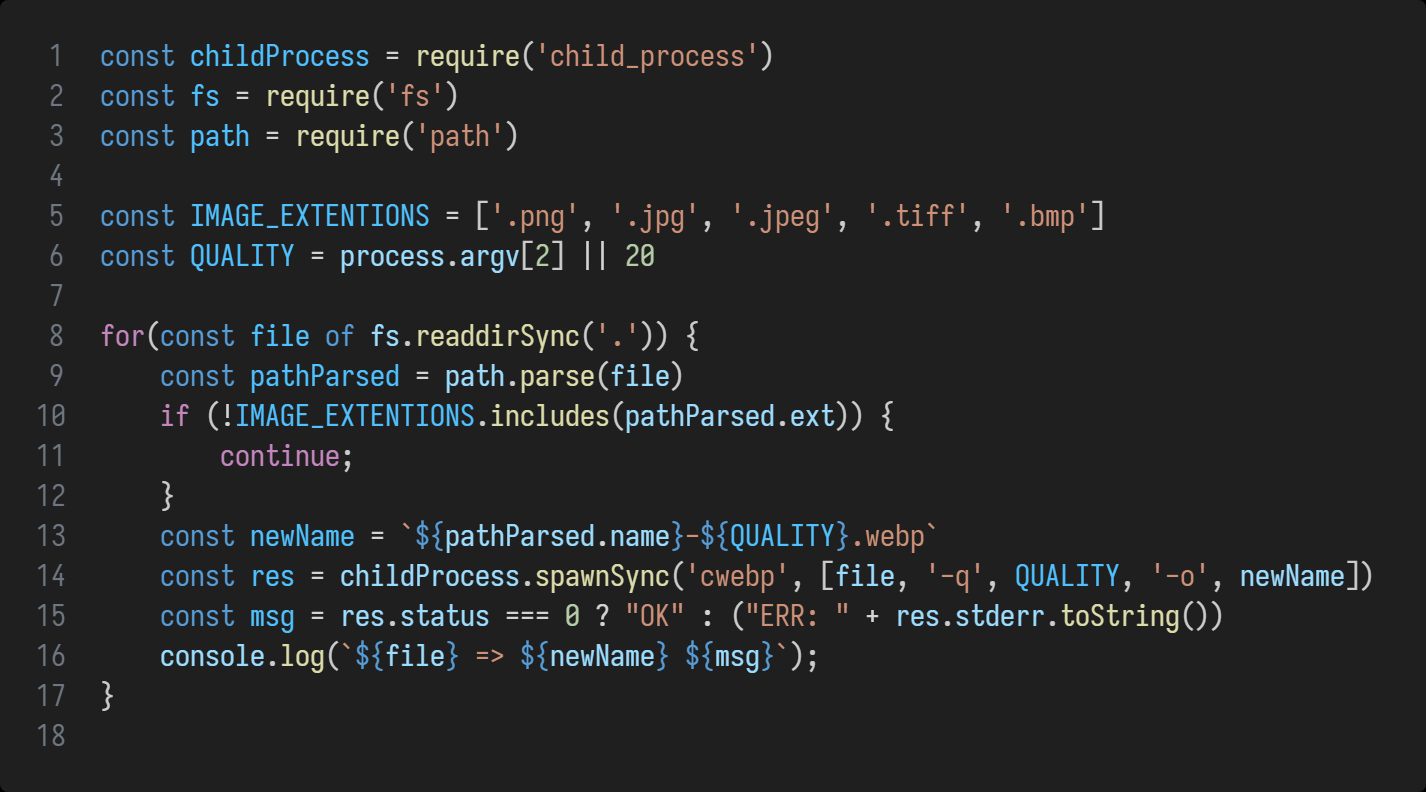
\includegraphics[width=\linewidth]{images/code_script_conv_webm.png}
  \caption{Skrypt konwertujący zdjęcia na format WebP}
  \label{fig:script-webp}
\end{figure}

Po uruchomieniu tego procesu w folderze ze zdjęciami, używając domyślnego parametru jakości równego 20, wygenerowane zostały nowe wersje wszystkich plików zdjęć na stronie. Finalny ich łączny rozmiar to $794.5$KB. W porównaniu do wcześniejszych $46.6$MB, jest to zmniejszenie o $98.3\%$, co jest wielką poprawą.

Możemy więc przetestować wpływ na wczytywanie witryny, przeprowadzając test WebPageTest'u.

\begin{figure}[H]
  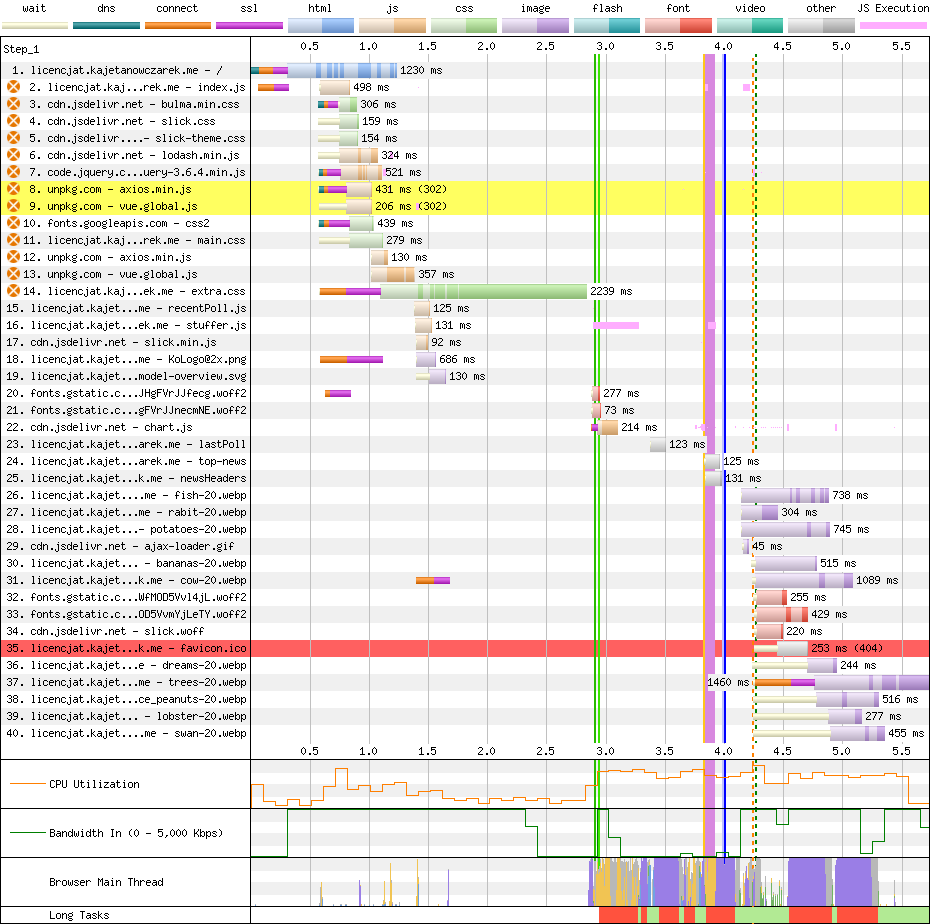
\includegraphics[width=\linewidth]{images/waterfall-after-webp.png}
  \caption{Wyniki testu po zmianie formatu zdjęć z PNG na WebP}
  \label{fig:waterfall-after-webp}
\end{figure}

Jak widać, zminiejszenie rozmiaru zdjęć o ponad $98\%$ odbiło się na czas wczytywania równie intensywnie, co wartość procentowa by sugerowała. Łączny czas wczytywania strony spadł z ponad $82$ sekund do $5.7$ sekundy. Niezmiennie, teraz, kiedy wykres nie jest zdominowany przez wczytywanie zdjęć na końcu procesu ładowania witryny, możemy zauważyć detale tego, co dzieje się w piewszych sekundach po nawigowaniu na naszą stonę.

\section{Analiza wczytywania 2}
Dzięki przeskalowaniu naszego wykresu, możemy ujrzeć dwa elementy, które wcześniej były zbytnio ściśnięte. Są nimi wcześniej wspomniane pionowe kreski oraz cieńkie elementy wierszy wykesu, repezentujące nawiązywanie połączeń i wykonywanie kodu JavaScript.

Zacznijmy od opisania, co reprezentują pionowe znaczniki. //todo opisać je

// TODO Napisać o połączeniach, przełączyć na h2

%Żeby nabrać pewnej intuicji, jak wiele więcej miejsca zajmują zasoby w porównaniu do kodu, zróbmy pewne porównanie. Według zainstalowanego na mojej maszynie Windows'a 11, pliki systemu operacyjnego zajmują $28.3\text{GB}$. W takiej samej ilości danych moglibyśmy zmieścić:

% \begin{center}
%   \begin{tabular}{|c|c|c|}
%     \hline
%     Rodzaj treści & Ilość treści & Rozmiar jednostki \\
%     \hline
%     Anglojęzyczna wikipedia\footnotemark[3] & 1.333 & 21.23GB \\ 
%     Niekompresowane audio jakości CD & 44.6 godzin & 1411 Kbit/s \\
%     Niekompresowane wideo HD (720p 30fps) & 409 sekund & 553 Mbit/s \\
%     Niekompresowane dane ekranu iPhone 14 Pro & 20.8 sekund & 1.36 GB/s \\
%     \hline
%   \end{tabular}
% \end{center}


\footnotetext[3]{Skompresowana, rozmiar z \url{https://en.wikipedia.org/wiki/Wikipedia:Size_of_Wikipedia}}


\vspace{5em}

\begin{itemize}
  \item Lepsze zdjęcia, format, rozmiary
  \item Kompresja i h2
  \item Async wczytywanie wielkich treści
  \item Obcinanie bibliotek JS/CSS
  \item Unikanie dużych bibliotek do prostych rzeczy
\end{itemize}


\chapter{Zakończenie}


\begin{thebibliography}{7}
\addcontentsline{toc}{chapter}{Bibliografia}
%
\bibitem{Lang}
Serge Lang, 
\textit{Algebra. Revised third edition}, 
New York, Springer-Verlag, 2002.
%
\bibitem{Kostrykin} 
Aleksiej Kostrykin, 
\textit{Wstęp do algebry. Podstawy algebry},
Warszawa, Wydawnictwo Naukowe PWN, 2022.
\end{thebibliography}
\end{document}